\documentclass[12pt]{article}
\setlength{\oddsidemargin}{0in}
\setlength{\evensidemargin}{0in}
\setlength{\textwidth}{6.5in}
\setlength{\parindent}{0in}
% \setlength{\parskip}{\baselineskip}
\usepackage{graphicx}
\usepackage{multirow}
\usepackage{multicol}
\usepackage{listings}
\usepackage{color}
\rmfamily
\definecolor{dkgreen}{rgb}{0,0.6,0}
\definecolor{gray}{rgb}{0.5,0.5,0.5}
\definecolor{mauve}{rgb}{0.58,0,0.82}

\lstset{frame=tb,
  language=R,
  aboveskip=3mm,
  belowskip=3mm,
  showstringspaces=false,
  columns=flexible,
  basicstyle={\small\ttfamily},
  numbers=none,
  numberstyle=\tiny\color{gray},
  keywordstyle=\color{blue},
  commentstyle=\color{dkgreen},
  stringstyle=\color{mauve},
  breaklines=true,
  breakatwhitespace=true,
  tabsize=3
}

\usepackage{amsmath,amssymb,amsrefs}
\usepackage[top=24mm, bottom=18mm, left=15mm, right=13mm]{geometry}
\usepackage{url}

\begin{document}
1. Considering the Laplacian denoted by $L$, then $G$ can be shown to be $k$-connected components if there $L$ can be broken into $k$ block diagonal matrices, which we can denote as $L_1, L_2,\dots,L_k$. That is:
\[ L = 
\begin{bmatrix}
L_1 & 0 & \dots & 0 \\
0 & L_2 & \ddots & 0 \\
\vdots & \ddots & \ddots & 0 \\
0 & \dots & \dots & L_k \\
\end{bmatrix}
\]
This is true since if there are separate components, then there is no edge between these components, so adjacency between points of different components should be 0. \\
Now by the property of Laplacians, the row sum and column sum of L is zero, so for all $L_1, L_2, \dots, L_k$, their row sums and column sums is 0. Thus, each have $\lambda_0 = 0$ with eigenvector $v_0 = (1,1,\dots, 1)$. Since there are $k$ blocks, each with 1 eigenvalue 0, and since $det(L) = det(L_1)det(L_2)\dots det(L_k)$, then $L$ has k components which is the multiplicity of the eigenvalue 0. 
\newpage
2.
\begin{lstlisting}
EnglandTeams = read.csv("England_2009_2010_TeamNames.csv", header = FALSE);
EnglandTeamScores = read.csv("England_2009_2010_Scores.csv", header = FALSE);

n = dim(EnglandTeamScores)[1];
S_match = (matrix(20, nrow=n, ncol=n) + as.matrix(EnglandTeamScores) %*% as.matrix(t(EnglandTeamScores)))/2;

D = diag(rowSums(S_match));

Laplacian = D - S_match;

E = eigen(Laplacian);
Ranking = E$vectors[,n-1];
Ranked = data.frame(Ranking, row.names = EnglandTeams[,1]);
Ranked[order(-Ranked$Ranking), , drop = FALSE];
\end{lstlisting}
This gives us the following ranking:\\ \\
\begin{tabular}{|c|c|}
\hline
'Burnley'     & 0.477379966\\
'Hull'        & 0.374209712\\
'Wigan'       & 0.285469630\\
'Portsmouth'  & 0.183143343\\
'Wolves'      & 0.183123190\\
'Sunderland'  & 0.119239116\\
'West Ham'    & 0.091111123\\
'Birmingham'  & 0.017176251\\
'Bolton'      & 0.014844431\\
'Stoke'       & 0.010421174\\
'Fulham'      & 0.002628019\\
'Blackburn'   &-0.002718788\\
'Liverpool'   &-0.084034033\\
'Aston Villa' &-0.099229806\\
'Everton'     &-0.157429641\\
'Arsenal'     &-0.174783324\\
'Tottenham'   &-0.273562003\\
'Man United'  &-0.291213755\\
'Chelsea'     &-0.329805720\\
\hline
\end{tabular}
\newpage
3a.\\
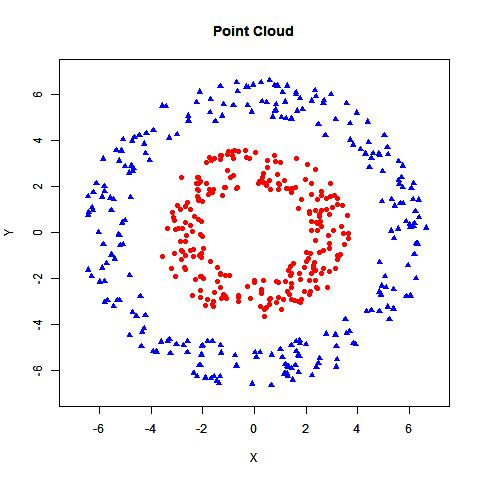
\includegraphics[scale = .65]{pointCloud.jpeg} \\
3b. \\
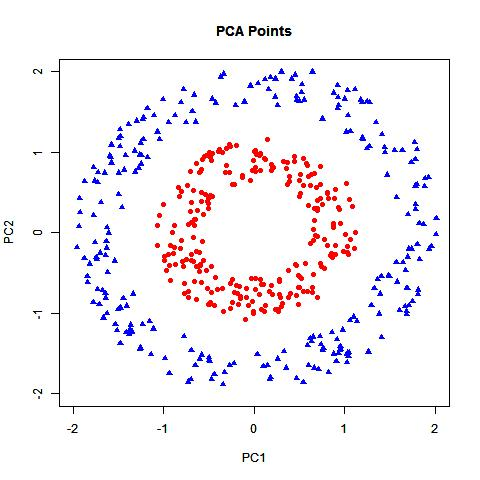
\includegraphics[scale = .65]{PCApoints.jpeg}
\newpage
3c.
\begin{lstlisting}
DIST = as.matrix(dist(A, method = "euclidean", diag = FALSE, upper = TRUE, p = 2));
W = exp(-DIST^2/1); #(.75,1)
D = diag(rowSums(W));
invD = solve(D);
L = invD %*% W;

# Obtain square root of D
eigD = eigen(D);
sqrtD = eigD$vectors %*% diag(sqrt(eigD$values)) %*% t(eigD$vectors);

S = sqrtD %*% L %*% solve(sqrtD);
eigS = eigen(S);
#Our result is the two eigenvectors eigS$vectors[,2], eigS$vectors[,3]
\end{lstlisting}
Graphs: \\
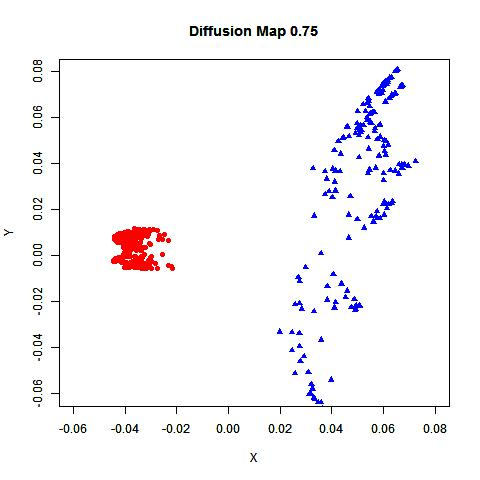
\includegraphics[scale = .55]{DiffusionMap075.jpeg}
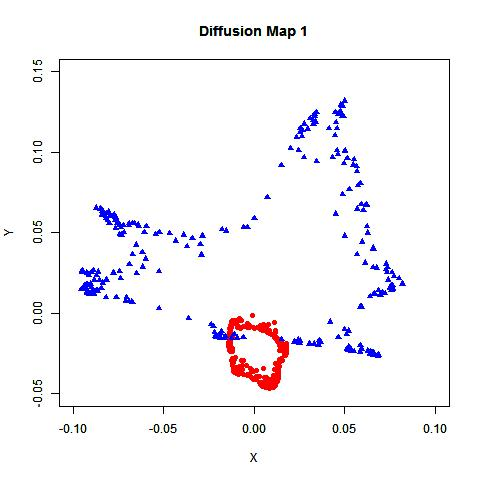
\includegraphics[scale = .55]{DiffusionMap1.jpeg} \\
The embedding with $\epsilon = 0.75$ has clearly separated clusters of the two circles. It gives a more readable representation of the relation of the two circles.
\newpage
4. \[\min_{x\in\mathbb{Z}_2^n}\sum_{(i,j)\in E}(x_i  - A_{ij}x_j)^2 = \min_{x\in\mathbb{Z}_2^n}x^T(D-A)x\] 
The matrix $(D-A)$ takes the form: \[
D - A = \left\{
\begin{array}{@{}l@{\thinspace}l}
\sum_{j=1,j \neq i}^n|A_{ij}| &: i = j \\
-A_{ij} &: i \neq j \\
\end{array}
\right\}
\]
Then $x^T(D-A)$ can be represented as the positive/negative sum column sum of $D-A$, depending on $x$. that is:
\[
x^T(D-A)_k = \sum_{j=1,j \neq i}^nx_j|A_{ij}|+\sum_{i=1,j\neq i}^n-x_iA_{ij}
\]
Finally, multiplying the vector x results in a summation of the positive/negative sum.
\[
\min_{x\in\mathbb{Z}_2^n}x^T(D-A)x =\min_{x\in\mathbb{Z}_2^n}\sum_{i=1}^nx_i(\sum_{j=1,j \neq i}^nx_j|A_{ij}|+\sum_{i=1,j\neq i}^n-x_iA_{ij})
\]
Combining the inner sums we get:
\[
\min_{x\in\mathbb{Z}_2^n}x^T(D-A)x = \min_{x\in\mathbb{Z}_2^n}\sum_{i,j\in E}x_i^2 -2\sum_{i,j\in E}A_{ij}x_ix_j + \sum_{i,j\in E}(A_{ij}x_j)^2
\]
Again, combining the sums gives us:
\begin{align} \nonumber
\min_{x\in\mathbb{Z}_2^n}x^T(D-A)x &= \min_{x\in\mathbb{Z}_2^n}\sum_{i,j\in E}x_i^2 -2A_{ij}x_ij_i + (A_{ij}x_j)^2 \\ \nonumber
\min_{x\in\mathbb{Z}_2^n}x^T(D-A)x &= \min_{x\in\mathbb{Z}_2^n}\sum_{i,j\in E}(x_i - A_{ij}x_j)^2
\end{align}
\end{document}
